\section{Ausgangslage}
\setauthor{Felix Dumfarth}
Zahlreiche Organisationen bauen heutzutage auf eine starke Webpräsenz und wickeln darauf komplexe Produkt- oder Leistungsfunktionalitäten ab.
Eine wichtige Rolle spielt dabei nicht nur der Kundenservice, sondern auch die Kommunikation, denn die Nutzer erwarten eine möglichst zeitnahe Beratung.
Die Bereitstellung von solchen Services ist derzeit mit hohen Kosten verbunden.

\section{Istzustand}
\setauthor{Felix Dumfarth}
Es gibt viele Personen die an der HTL Leonding interessiert sind und sich gerne schnell über die Schule informieren wollen.


\section{Problemstellung}
\setauthor{Felix Dumfarth}
Die HTL Leonding hat ein großes Informationsangebot, zu diesem gibt es viele Zugänge, zum Beispiel auf der Webseite ist es oft schwierig den Überblick zu bewahren mit den vielen Unterseiten und daher wäre eine Unterstützung zum Finden für die vielen Informationen hilfreich.

\section{Aufgabenstellung}
\setauthor{Felix Dumfarth}
In dieser vorliegenden Arbeit soll ein Chatbot für die HTL Leonding Webseite erstellt werden, der Besuchern der Webseite einfach und schnell schulspezifische Fragen beantworten soll.
Jedoch soll es auch möglich sein, dass der Bot auch als Grundlage für weitere Arbeiten in der Schule, wie zum Beispiel der 3D Leonie, zum Einsatz kommen kann.

\section{Use-Cases}
\setauthor{Felix Dumfarth}

\begin{figure}[hbt!]
    \centering
    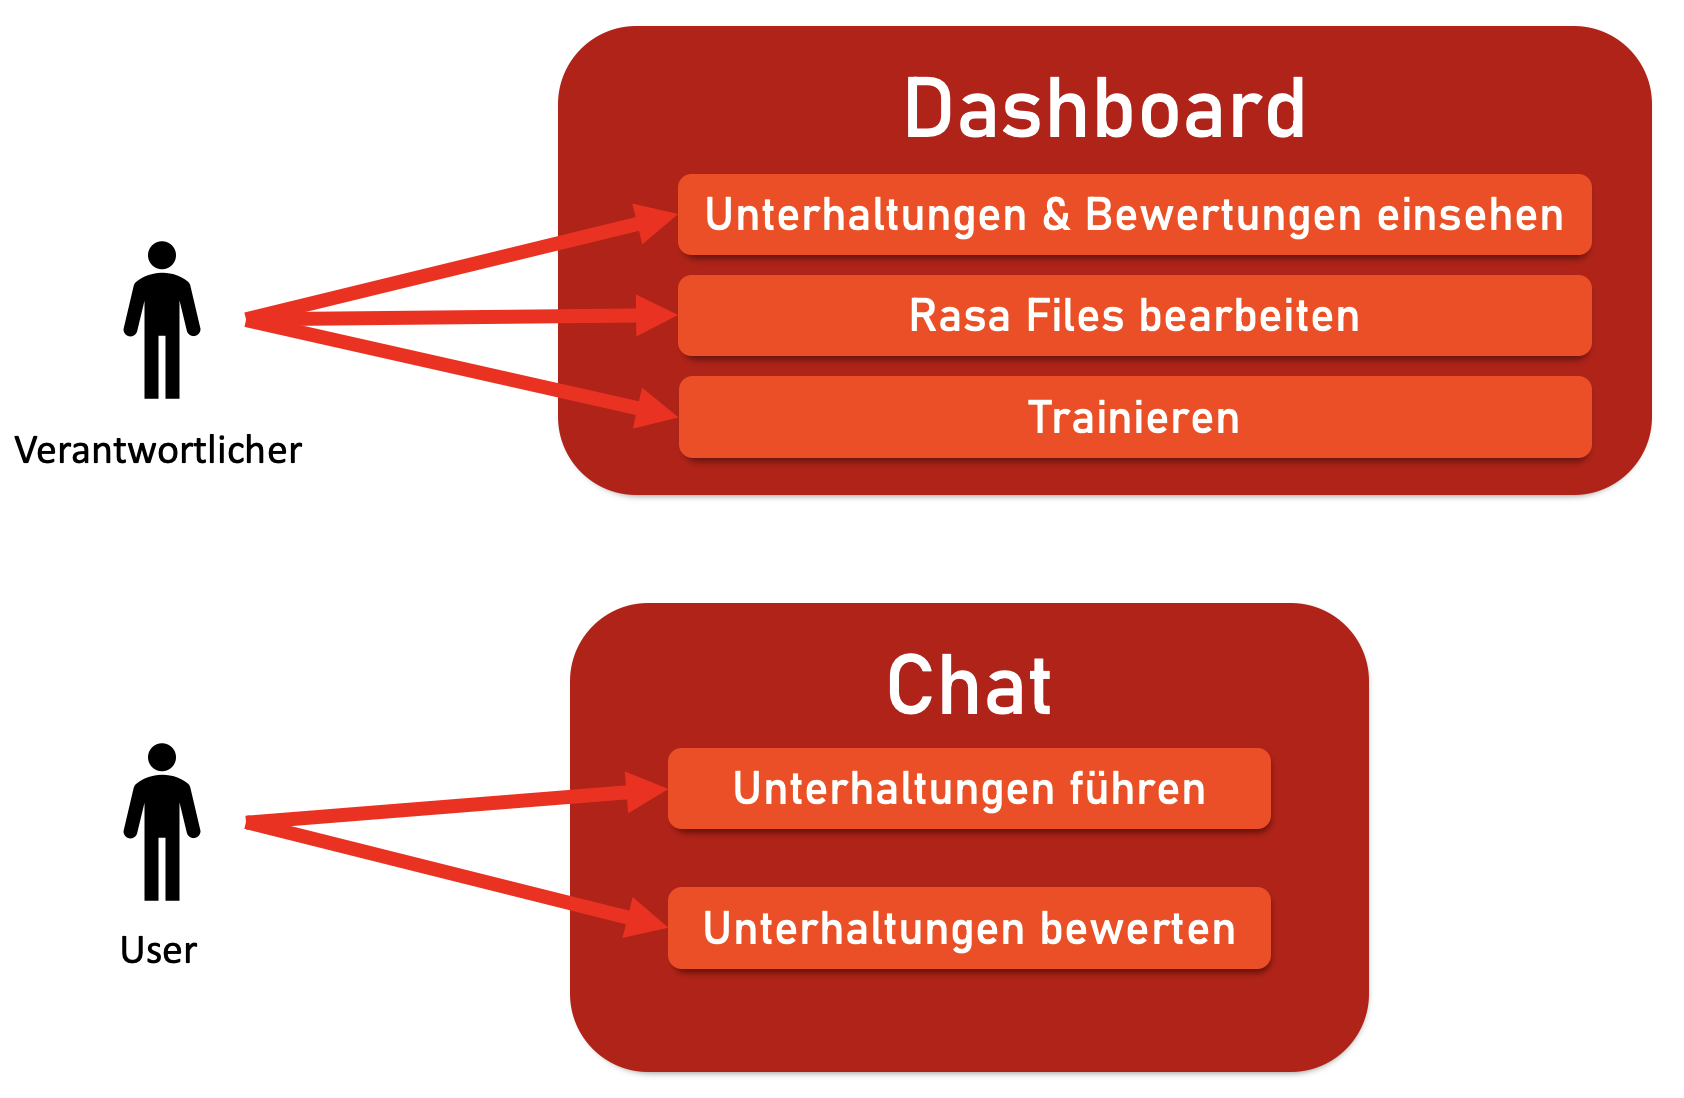
\includegraphics[scale=0.5]{pics/usecase}
    \caption{Use-Case Diagramm}
    \label{fig:impl:usecase}
\end{figure}

Der User kann hauptsächlich schulspezifische Unterhaltungen mit dem Chatbot führen und diese Unterhaltung anhand ihrer Qualität bewerten.
Eine verantwortliche Person kann sich die Unterhaltungen und Bewertungen von Usern ansehen, sodass Sie diese beurteilen kann.
Außerdem kann die verantwortliche Person die Rasa Files, nlu.yml, stories.yml, rules.yml und domain.yml bearbeiten und den Chatbot auffordern sein neues Wissen zu trainieren.
